\documentclass[compress,handout,10pt]{beamer}

\newlength{\wideitemsep}
\setlength{\wideitemsep}{\itemsep}
\addtolength{\wideitemsep}{100pt}
\let\olditem\item
\renewcommand{\item}{\setlength{\itemsep}{0.5\baselineskip}\olditem}

\usetheme{berlin}
\usecolortheme{orchid}
\usefonttheme[onlymath]{serif}

\setbeamertemplate{bibliography item}[text]
\usepackage{float}
%\floatstyle{boxed}
\usepackage{colortbl}
\usepackage{mathpazo}
\usepackage{graphicx}
\graphicspath{{./extra/}}
\usepackage{movie15}
\usepackage{bm}
\usepackage{verbatim}
\usepackage{comment}
\usepackage [font=small, labelfont=bf]{caption}
\usepackage{subcaption}
%\captionsetup[subfigure]{labelformat=empty}
\captionsetup[figure]{labelformat=empty}

\newcommand{\mygreen}{\color{green!50!black}}
\newcommand{\myblue}{\color{blue}}
\newcommand{\myred}{\color{red}}
\newcommand{\mycolor}{\color{red}{c}\color{blue}{o}\color{green}{l}\color{orange}{o}\color{cyan}{r}}
\newcommand{\mysize}{\scriptsize{s}\small{i}\normalsize{z}\Large{e}}
\newcommand{\myshape}{\textcircled{s}\textit{h}\texttt{a}\textsf{p}\textsc{e}}

%\xdefinecolor{titlecolor}{rgb}{.855,.647,.125}
%\xdefinecolor{titlecolor}{rgb}{0,0,0}
%\setbeamercolor{frametitle}{fg=titlecolor}
\setbeamerfont{frametitle}{series=\bfseries}
\setbeamercolor{normal text in math text}{parent=math text}

\setbeamertemplate{navigation symbols}{} %gets rid of navigation symbols
\setbeamertemplate{footline}[frame number]
\beamertemplateshadingbackground{blue!5}{yellow!10}

\title{{\LARGE Modeling and Simulating Fan Participation at Large Scale Sporting Events\newline} }

\subtitle{{\large Blue Jays Unlimited} }

\author{ 
%    \vspace{5pt}
    {\bf{Presenters:}}\\ 
Ahmed Aly\\
Steven Su \\
Danni Tang\\ 
    \vspace{5pt}
} 
\institute{JHU AMS 550.400 Fall 2012}
\date{Last Complied on \today} 

\begin{document}

\begin{frame}[plain]
	\titlepage
\end{frame}

\begin{frame} [allowframebreaks]
	\frametitle{Overview}
{\small \tableofcontents}
\end{frame}

\section{Introduction}

\subsection{Importance of Cheering}

\begin{frame}
	\frametitle{The Importance of Cheering in Sports}
		\begin {itemize}
			\item A loud and supportive home crowd is the ultimate home team advantage for sports teams
			\item Home crowd advantage effects the result of the game, shown by past research:
			\begin{itemize}
				\item In US professional sporting leagues, home teams can win approximately 60\% of the time \cite{Jamieson_2010}
				\item In US college athletics, home teams can win approximately 66\% of games player \cite{Snyder_1985}
			\end{itemize}
		\end {itemize}
\end{frame}

\begin{frame}
	\frametitle{What is Cheering?}
		\begin{itemize}
		\item Home crowd can also improve the ambiance of a sporting event
		\item Can show support and enhancing the atmosphere by "cheering":
		\begin{itemize}
			\item Chanting the school fight song
			\item Waving a rally towel
			\item Doing the wave
			\item Clapping in general
		\end{itemize}
	\item Cheering is essential at collegiate sporting events; improves experience for both teams and the fans
	\end{itemize}
\end{frame}

\subsection{The Johns Hopkins Blue Jays}

\begin{frame}
	\frametitle{The Johns Hopkins Blue Jays}
		\begin{itemize}
			\item The Blue Jays have amassed 47 national championships and 187 conference titles.\cite{hopathletic}
			\item The Blue Jays have excelled at many sports including:
			\begin{itemize}
				\item The Men's Lacrosse team has won 44 national championships, most recently in 2007.\cite{hopathletic}
				\item The Men's Swimming team won 32 conference championships, including a streak of 28 consecutive conference championships from 1971-1998.\cite{hopathletic}
				\item The Men's Football and Baseball teams were each conference champions for three consecutive years from 2009-2011. \cite{hopathletic}
		\end{itemize}
	\end{itemize}
\end{frame}

\subsection{Sponsor Information}

\begin{frame}
	\frametitle{Who are Blue Jays Unlimited?}
		\begin {columns}
			\begin{column}{0.5\textwidth}
				\begin {itemize}
					\item Blue Jays Unlimited (BJU) was established in 1995 \cite{bjuwebsite} by a volunteer group of alumni, friends, and staff
					\item Has more than 3000 active members dedicated to supporting and promoting Johns Hopkins University (JHU) athletics \cite{bjuwebsite}
					\item Official booster club for JHU athletics \cite{bjuwebsite}
				\end {itemize}
			\end {column}
			\begin {column}{0.5\textwidth}
				\begin{figure} [h]
					\begin{center}
						
\includegraphics [width=2in] {BJU.jpg}
						\caption {{\tiny The logo of Blue Jays Unilimited. \textit{Courtesy of: http://www.hopkinssports.com/bluejays-unlimited/}}}
					\end{center}
				\end {figure}
			\end {column}
		\end{columns}
\end{frame}

\begin{frame}
	\frametitle{What Does BJU do for Hopkins?}
	\begin {columns}
		\begin {column} {0.5\textwidth}
		\begin {itemize}
			\item Raised more than \$4 million in funds to improve experience for JHU student athletes and fans alike \cite{bjuwebsite}
			\item Funds provide money for capital projects as well as scholarships and operational endowments \cite{bjuwebsite}
			\item Past projects include renovation of the Newton H.~White Athletic Center and recognition banners for championship teams. \cite{bjuwebsite}
		\end {itemize}
	\end {column}
	\begin{column} {0.5\textwidth}
		\begin{figure}
			\begin{center}
				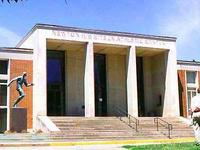
\includegraphics [width=2in] {AthleticCenter.jpg}
				\caption{{\tiny The Newton H.~White Athletic Center after renovations. \textit{Courtesy of: http://events.jhu.edu/WhiteAthleticCenter\#.UHhNK1GRWSo}}}
			\end{center}
		\end {figure}
	\end {column}
\end {columns}
\end {frame}

\begin{frame}
\frametitle{BJU at Sporting Events}
\begin{itemize}
\item BJU is present at nearly all major JHU sporting events
\item Encourage fans to cheer on their Blue Jays to victory in a vociferous and family-friendly manner
\item BJU is interested in maximizing the amount of fan participation in cheering at sporting events to provide the ultimate advantage: a spirited home crowd
\item They believe they can increase fan participation in cheering events by strategically placing ``cheer starters"--student volunteers who lead and urge other fans around them to cheer
\end{itemize}
\end{frame}

\section{Problem Statement}

\subsection{Problem Statement Background}

\begin{frame}
	\frametitle{Problem Statement Background: Why is Cheering Important?}
	\begin{itemize}
	\item A loud and supportive home crowd is the ultimate home team advantage to any collegiate sports team.
	\item Fan participation in events such as chanting the school fight song, waving a rally towel, doing the wave, or general applause, show support for the home team as well as enhance the general atmosphere of a sporting event.
	\item Note that we will hence refer to all these activities as ``cheering''.
	\end{itemize}
\end{frame}

\subsection{Official Problem Statement}

\begin{frame}
	\frametitle{Official Problem Statement}
		\begin{itemize}
			\item BJU wants to know if ``cheer starters'' can actually increase cheering and also want a simple model of fan participation in cheering.
		\end{itemize}
\end{frame}

\section {Objectives}

\begin{frame}
	\frametitle{Objective Statements}
		\begin{itemize}
			\item Our task is to provide BJU with a simple model of fan participation in cheering at Homewood Field
			\item We will also provide simulation results from the model which determine if their belief about cheer starters is accurate
			\item If cheer starters are effective, and time permitting, we will provide BJU with details about the quantity and location at which cheer starters should be placed in order to maximize cheering
		\end{itemize}
\end{frame}

\subsection{Important Details to Consider}

\begin{frame}
	\frametitle {Important Details To Consider}
	\begin {columns}
		\begin {column}{0.5\textwidth}
		\begin{itemize}
			\item Homewood Field's capacity is approximately 8500 spectators \cite{wiki}
			\item Long rectangular section of the bleachers in the lower left is traditionally reserved for Blue Jays' fans and seats approximately 4000 fans.
		\end {itemize}
	\end {column}
	\begin {column}{0.5\textwidth}
	\begin {figure}
	\begin{center}
		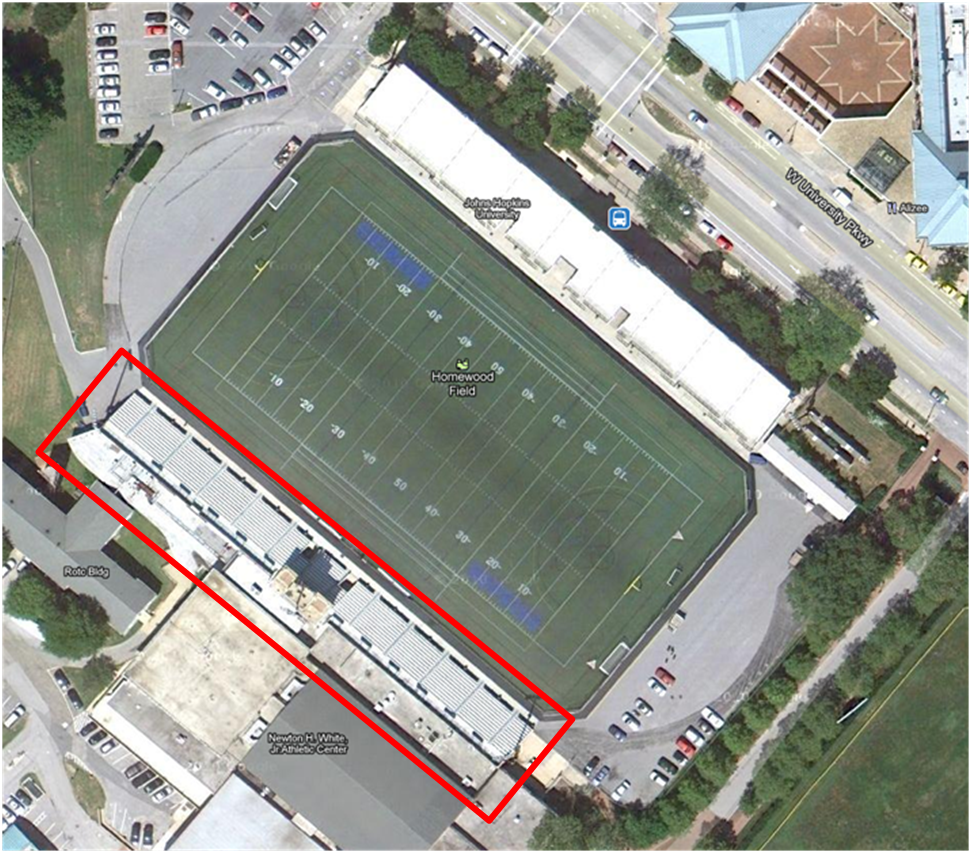
\includegraphics [width=2in] {Bleachers.png}
		\caption {{\tiny A satellite image of Homewood Field. The home team bleachers are highlighted in red. \textit{Courtesy of: www.google.com}}}
		\end{center}
	\end{figure}
\end {column}
\end {columns}
\end{frame}


\begin{frame}
	\frametitle{Important Details to Consider}
	\begin{itemize}
		\item Home bleachers are usually filled to capacity for all major Hopkins sporting events
		\item Because of how fans normally sit, BJU is specifically interested in maximizing cheering in the home team bleachers
	\end{itemize}
\end{frame}

\subsection{Official Objectives}

\begin{frame}
	\frametitle {Official Objectives}
	\begin {itemize}
		\item Our task is to provide BJU with a simple model of fan participation in cheering at Homewood Field in the home team bleachers as well as simulation results from the model which determine if their belief about cheer starters is accurate.
		\item If cheer starters are found to be effective, we will attempt to provide BJU with more details about the quantity and location at which cheer starters should be placed in order to maximize cheering.
		\end {itemize}
\end{frame}

\section{Analysis and Simualtion}
\begin{frame}
\frametitle{Simplifications and Assumptions}
\begin{itemize}
	\item The willingness of a fan in a crowd to cheer depends on the number of people cheering around the given fan and how long the surrounding people have been cheering. 
	\item The greater the number of people surrounding a fan who are cheering, and the longer the surrounding people have been cheering, the more likely that fan will start to cheer.
	\item The innate support level a fan has for the team also influences the willingness of that fan to start cheering.
	\item A cheering fan continues cheering until the end of the simulation.
	\item The performance of the sports team does NOT influence cheering.
	\end{itemize}
\end{frame}

\subsection{Comptutational Simulation}

\begin{frame}
\frametitle{ Step 1: Generating Innate Support Level}
\begin{itemize}
\item We generate an arbitrary sized $n$ x $m$ matrix,
\item  $X$, to represent a $nm$ sized crowd.
\item   $X_{ij}$ represents fan $ij$. Each element in $X$ corresponds to fan's innate support level for the team.
Innate support level was generated by sampling from a normal random distribution with a mean of 10 and a standard deviation of 1 as shown in (\ref{1}).
\end{itemize} 
\begin{equation}
X_{ij}\sim Norm(10,1),~\forall~i\in[1,n],~j\in[1,m]
\label{1}
\end{equation}
\end{frame}

\begin{frame}
\frametitle{Step 2: Determinining Which Fans are Initially Cheering}
\begin{itemize}
\item Set an initial threshold, $T_{init}$ to determine which of the fans in the matrix are \textit{initially} cheering.
\item A new $n$ x $m$ matrix, $X'$, with each element in $X'$ is initially assigned a value of 1, if the corresponding element in $X$ had a value which was greater than or equal to the initial threshold, otherwise the element is given a value of 0. See (\ref{2}). 
\item $X'$ is the matrix used to keep track of who is cheering. (1=cheering, 0=not cheering). 
\end{itemize}
\begin{equation}
X'_{ij}=1~if~X_{ij}\geq T_{init},~X'_{ij}=0~if~X_{ij}<T_{init}
\label{2}
\end{equation}
\end{frame}


\begin{frame}
\frametitle{Step 3: Including the Influence of Surrounding Fans}
\begin{itemize}
\item $S$ is a $n$ x $m$ matrix stores how many people surrounding a given fan are cheering at a given time.
\item Each element in $S$ has corresponding elements with the same row and column indices in both $X$ and $X'$, all of which store different model values for the same individual fan. 
\item Define a round, $r$, to be the passing of an arbitrary time interval (approximately 3-5 seconds, in this case). 
\item $Y$is an $n$ x $m$ matrix compute the individual elements of $Y$ according to (\ref{3}). 
\end{itemize}
\begin{equation}
Y_{ij}=X_{ij}(S_{ij})+r,~\forall~i\in[1,n],~j\in[1,m]
\label{3}
\end{equation}
\item Note:By computing $Y$ as shown in (\ref{3}), the likelihood of a fan starting to cheer increases with the number of surrounding fans who are cheering as well as with the length of time those fans have been cheering(greater $R$ value).
\end{frame}

\begin{frame}
\frametitle{Step 4: Updating Matrices and Comparing to Absolute Threshold}
\begin{itemize}
\item Each element in $Y$ represents an individual fan and has corresponding elements in $X$, $X'$, and $S$, with the same row and column indices. 
\item Elements in $Y$  are compared to an absolute threshold, $T_{absolute}$.
	\begin{itemize} 
		\item If an individual's score in $Y$ is greater than or equal to the absolute threshold, the individual will begin to cheer, and we set the corresponding element in $X'$ equal to 1. This is shown in (\ref{4}).
		\begin{equation}
			X'_{ij}=1~if~Y_{ij}\geq T_{absolute}
			\label{4}
		\end{equation}
		\item If the individual's score in $Y$ is less than the absolute threshold, corresponding element in $X'$ remains 0.  
\end{itemize}
\end{itemize}
\end{frame}

\begin{frame}
\frametitle{Step 5: Repeating Rounds}
To simulate the passing of time:
	\begin {enumerate}
		\item Setup matrices with appropriate initial conditions (i.e.~randomly assign innate support levels to each fan and choose quantity and location of cheer starters)
		\item Check to see if any new fans join cheering
		\item Update matrices (i.e.~$X'$ and $Y$)
		\item Repeat for $R$ rounds
	\end {enumerate}
\end{frame}

\section{Results}

\begin{frame}
	\frametitle{Final Parameters}
	\begin{itemize}
		\item Rows, $n=20$
		\item Columns, $m=100$
		\item Initial Threshold, $T_{init}=11$
		\item Absolute Threshold, $T_{absolute}=46$
		\item Rounds, $R=10$
		\item Number of Cheer Starters, $CS$ (Variable)
	\end{itemize}
\end{frame}

\begin{frame}
	\frametitle{Monte Carlo Simulation}
	\begin{itemize}
		\item For a given $CS$ value, the $CS$ cheer starters were randomly placed in the crowd. The crowd simulation was then ran and the final percentage of cheering fans after 10 rounds was computed as previously described.
		\item For a given $CS$ value this was procedure was repeated for 1000 trials (Monte Carlo Simulation) and the average final percentage of cheering fans after 10 rounds over the 1000 trials was computed. 
		\item Repeated this for $1 \leq CS \leq 50$.
		\item The average final percentage of cheering fans for each $CS$ value was compared to that of when $CS=0$ using a t-test. 
	\end{itemize}
\end{frame}

\begin{frame}
	\frametitle{$CS\geq 39$ Produces Statistically Significant Increase in Cheering}
	\begin{itemize}
		\item When $CS\geq39$, there is a statistically significant $(p<0.05)$ increase in the average final percentage of the crowd who are cheering
		\item If $CS$ is increased further, the final percentage of the crowd cheering increases, and the p-value decreases
	\end{itemize}
\end{frame}

\begin{frame}
	\frametitle{Final Percent of Crowd Cheering vs Number of Cheer Starters}
	\begin{figure} [h]
		\begin{center}
    			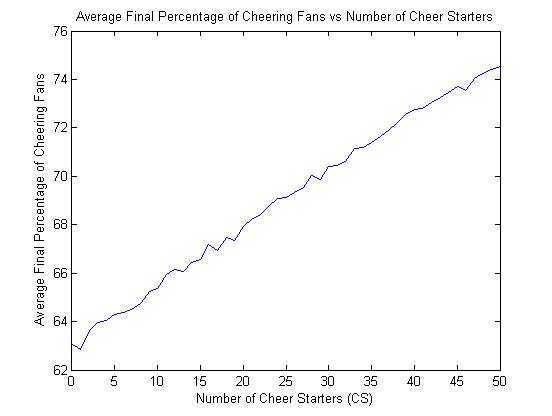
\includegraphics [width=3in] {46(1).jpg}
    			\caption {{\tiny Final cheering percentage for various $CS$ values.}}
    		\end{center}
    	\end {figure}	
\end{frame}

\begin{frame}
	\frametitle{Percent of Crowd Cheering Over Time For Various $CS$}
	\begin{figure} [h]
		\begin{center}
    			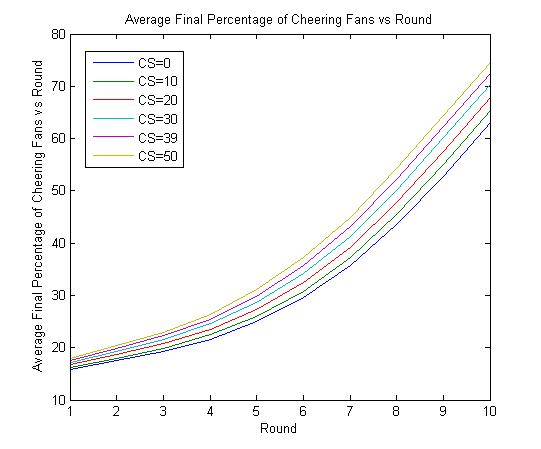
\includegraphics [width=3in] {46(2).jpg}
    			\caption {{\tiny Percent of crowd cheering over time for various $CS$ values.}}
    		\end{center}
    	\end {figure}	
\end{frame}

\begin{frame}
    \frametitle{Visualization of Cheering}
    \begin {columns}
    	\begin{column}{0.5\textwidth}
    		\begin{figure}
    		\begin{center}
    		  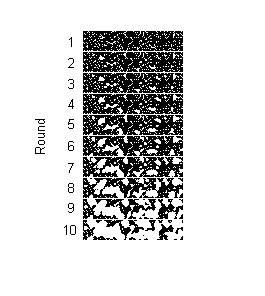
\includegraphics [width=2in] {n=0,46.jpg}
    			\caption {{\tiny Cheering over time when $CS=0$. White indicates cheering.}}
    			\end{center}
    		\end{figure}
    	\end {column}
    	\begin {column}{0.5\textwidth}
    	\begin{figure} [h]
    		\begin{center}
    			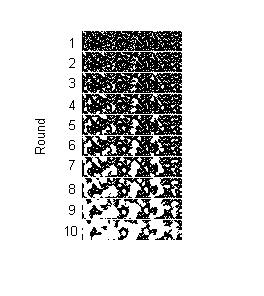
\includegraphics [width=2in] {n=39,46.jpg}
    			\caption {{\tiny Cheering over time when $CS=39$. White indicates cheering.}}
    		\end{center}
    	\end {figure}	
    	\end {column}
    \end{columns}
\end{frame}

\section {Deliverables and Timeline}

\subsection{Deliverables}

\begin{frame}
	\frametitle{Deliverables}
	The model will be coded on MATLAB R2009b. All computations will be performed on a Intel Core i7 Desktop PC. \newline
	\end{frame}

\begin{frame}
	\frametitle{Deliverables}
	From Team to Sponsor:
	\begin {itemize}
	\item MATLAB R2009b and R combination package. The model will be coded in MATLAB but a complete set of documentation will be provided in R. We will also generate some test scripts that can be used to reproduce our numerical and simulation test results
	\item If time permits, a list of patterns of cheer starter setups (i.e.~the number of cheer starters and location of them) that maximize fan cheering
	\item Technical report and presentations summarizing the work \newline
	\end{itemize}
\end{frame}

\begin{frame}
	\frametitle{Deliverables}
	From Sponsor to Team:
	\begin{itemize}
		\item Timely responses to inquiries
	\end{itemize}
\end{frame}

\subsection{Timeline}

\begin{frame}
	\frametitle{Timeline of Milestones}
	\begin{itemize}
    \item Work Statement due date, Sep 28, 2012.
    \item Midterm Presentation due date, Oct 17, 2012.
    \item Progress Report due date, Oct 26, 2012.
    \item Final Presentation due date, Nov 16, 2012.
    \item Final Report due date, Nov 30, 2012.
	\end{itemize}
\end{frame}

\section{Conclusion}

\subsection{Work Remaining to Be Done}

\begin{frame}
	\frametitle{Remaining Work}
	\begin {itemize}
		\item Begin coding the model in MATLAB.
		\item Run simulations using the model.
		\item Time permitting, try to find patterns in cheer starter setups which maximize cheering.
	\end {itemize}
\end{frame}

\subsection{Recommendations for Future Research}

\begin{frame}
	\frametitle {Recommendations for Future Research}
	\begin {itemize}
		\item It would be interesting to see if this model could be applied to other social events (concerts, college lectures, theaters, etc.) where there are large crowds and applause is relevant.
	\end {itemize}
\end{frame}

\subsection{}

\begin {frame} [allowframebreaks]
	\frametitle{References}
	\bibliographystyle{plain}
	%\nocite{*}
	\bibliography{extra/biblioWS}
\end {frame}

\begin{frame}
	\frametitle {Questions?}
	\begin{center}
		Questions?
	\end{center}
\end{frame}

\end{document}
\end{flushleft
